\section{Symbolske udtryk}
Det ønskes at kunne repræsentere simple udtryk som en type i F\#. Vi skal derfor gennemgå en del teori og funktioner som er nødvendige for at kunne dette. Det vil give os et grundlæggende fundament for at kunne udføre matematiske evalueringer som differentiering i F\#. Som de fleste andre programmer har F\# kun \texttt{float} og \texttt{int} som kan repræsentere tal. Derfor vil vi begynde med at definere et modul som indeholder en type for tal. Tankegangen her, er at gennemgå en opbygning af en repræsentation af udtryk, samt at kunne reducere dem. Vi begrænser os selv til at kun anvende matematiske operationer som addition, subtraktion, negation, multiplikation og division.

\subsection{Tal mængder}
Vi begynder med opbygningen af et modul, der kan repræsentere en talmængde. Typen for tal består af tre konstruktører, henholdsvis for heltal, rationale tal og komplekse tal hvor real- og imaginærdelen er rationale. 

\subsubsection{Rationale tal modul}\label{sec:rational}
Repræsentationen af rationale tal kan laves ved hjælp af et heltals talpar. Hvor det ene heltal er tælleren, og det andet er nævneren.

\begin{lstlisting}[language={FSharp}, 
    label={type_rationel},
    caption={Typen for rationale tal}]
type rational = R of int * int
\end{lstlisting}
Nedenfor er der givet en signaturfil for \texttt{rational} modulet Listing \ref{rational_fsi}. I implementeringsfilen overskrives de matematiske operatorer ved hjælp af de klassiske regneregler for brøker\footcitetitle{Rational_number}.

\lstinputlisting[
    language=FSharp,
    label={rational_fsi},
    caption={Signaturfilen for rational-modulet}
]{../modules/rational.fsi}
For at kunne sammenligne, samt for nemmere at undgå for store brøker, vil alle rationale tal blive reduceret til deres simpleste form. Dette gøres ved at finde den største fælles divisor (GCD) \footcitetitle{gcd}. Derudover er det vigtigt at være opmærksom på ikke at foretage nul division. Derfor vil implementeringsfilen kaste en "System.DivideByZeroException", hvis nævneren er eller bliver nul. Signaturfilen indeholder en række funktioner, som anvendes af andre filer. Det vil desuden være nødvendigt at kunne håndtere overflow. Idet heltallene, der repræsenterer de rationale tal, under eller efter operationen kan blive for store til korrekt at blive repræsenteret af 32-bit. Da denne rapport fokuserer på implementeringen af matematiske koncepter og ikke numeriske algoritmer, vil modulet blot slå en fejl, hvis der opstår overflow.
 


\subsubsection{Komplekse tal-modul}
Vi skal nu dykke lidt mere ned i implementeringen af et modul for komplekse tal. Signaturfilen \textit{complex.fsi} er givet i Appendiks \ref{sec:complex.fsi}. 

Først defineres en type for komplekse tal, som består af et rationelt tal par, henholdsvis for realdelen og imaginærdelen, se Listing \ref{type_complex}.

\begin{lstlisting}[language={FSharp}, 
    label={type_complex},
    caption={Typen for komplekse tal}]
type complex = C of rational * rational
\end{lstlisting}

Der kan opskrives en række regneregler i Definition \ref{def:complex} for operationer på komplekse tal. 
\vspace{0.5cm}
\begin{definition}[Regneregler for komplekse tal]\label{def:complex}
  Lad $a, b, c, d \in \mathbb{Q}$, så er følgende defineret omkring komplekse tal\footcitetitle[se. Definition 3.3 s. 54, Definition 3.5 s. 56, Definition 3.8 s. 57, ligning 3-2 s. 58]{mat1a}:
  \begin{enumerate}
    \item \textbf{Addition} \\ $(a + bi) + (c + di) = (a + c) + (b + d)i$
    \item \textbf{Subtraktion} \\ $(a + bi) - (c + di) = (a - c) + (b - d)i$
    \item \textbf{Multiplikation} \\ $(a + bi) \cdot (c + di) = (ac - bd) + (bc + ad)i$
    \item \textbf{Kvadratisk form} \\ $ (a + bi) \cdot (a - bi) = a^2 + b^2$
    \item \textbf{Konjugering} \\ $\overline{a + bi} = a - bi$
    \item \textbf{Division} \\ $\frac{a + bi}{c + di} = \frac{(a + bi)\cdot(c - di)}{c^2 + d^2}$
  \end{enumerate}
\end{definition}

For implementeringen af addition, subtraktion, multiplikation samt skalering med et rationelt tal, se Listing \ref{complex_operations}. Skaleringen af et rationelt tal, kan udledes fra multiplikation, ved at lade den imaginære del være $0$. Er det simple operationer, som ikke behøver at defineres i særskilte funktioner. De kan defineres direkte på overskrivningen af deres respektive operatorer. Dog er det nødvendigt at definere multiplikation som en funktion, da den skal anvendes af divisionsfunktionen. 
\begin{lstlisting}[language={FSharp}, 
    label={complex_operations},
    caption={Overskrivning af operationer på komplekse tal}]
// complexDivRational: complex -> rational -> complex
let complexDivRational c (n) = 
    match c with
    | _ when isZero n ->  raise (System.DivideByZeroException("Complex.divRational: Cannot divide by zero!"))
    | C(a, b) -> C(a / n, b / n) 

// mulConjugate: complex -> rational
let mulConjugate (C(a, b)) = a*a + b*b

// conjugate: complex -> complex
let conjugate (C(a, b)) = C(a, -b)

// mulComplex: complex -> complex -> complex
let mulComplex (C(a, b)) (C(c, d)) = C(a*c-b*d, b*c+a*d)

// divComplex: complex -> complex -> complex
let divComplex z1 z2 =
    complexDivRational (mulComplex z1 (conjugate z2)) <| mulConjugate z2

type complex with
    static member (+)  (C(a, b), C(c, d)) =  C(a + c, b + d)
    static member (-)  (C(a, b), C(c, d)) =  C(a - c, b - d)
    static member (*)  (n, C(a, b))       =  C(n * a, n * b)
    static member (*)  (C(a, b), n)       =  C(n * a, n * b)
    static member (*)  (z1, z2)           =  mulComplex z1 z2
    static member (/)  (z, n)             =  complexDivRational z n
    static member (/)  (z1, z2)           =  divComplex z1 z2 
    static member (~-) (C(a, b))          =  C(-a, -b)
\end{lstlisting}    

Bortset fra division af to komplekse tal, ligner de resulterende overskrivninger på operationerne deres respektive matematiske definitioner. Men når vi nærmere studerer divisionen af to komplekse tal, ser vi, at der blot er brug for få funktioner til at kunne udføre divisionen. Først konjugeres nævneren, derefter multiplikeres resultatet med tælleren. Til sidst divideres resultatet af multiplikationen med kvadratet af nævneren. Da komplekse tal som en talmængde indeholder heltal og rationale tal, vil vi i det følgende afsnit omkring tal-modulet anvende komplekse tal til udføre de matematiske operationer i modulet.


\subsubsection{Tal-modulet}
Vi har nu beskrevet en måde at kunne repræsentere brugerdefinerede tal på ved brug af typer i F\#. Det vil derfor være oplagt at have en type som indeholder alle de typer tal, vi ønsker at kunne anvende i de matematiske udtryk, vi er ved at opbygge. Fordelen ved at samle dem til en type er, at vi kan lave en række funktioner. Dette inkluderer blandt andet matematiske operationer, som kan anvendes på  vores typer for tal. Ved at samle dem til en type \texttt{Number} kan vi også opskrive en række egenskaber i \ref{egenskab:tal} som vi ønsker at de skal opfylde. Egenskaberne vil blive valideret ved brug af PBT i sektion \ref{sec:PBT_number}.

\vspace{0.5cm}
\begin{egenskab}[Egenskaber for \texttt{Number}-typen]\label{egenskab:tal}
  Lad $a, b, c \in \text{\texttt{Number}}$, så gælder følgende\footcitetitle[se. Side 124 Definition 6.1]{mat1a}:
  \begin{enumerate}
    \item Addition og multiplikation er \textbf{associative} \\ $a + (b + c) = (a + b) + c$ og $a \cdot (b \cdot c) = (a \cdot b) \cdot c$
    \item Addition og multiplikation er \textbf{kommutative} \\ $a + b = b + a$ og $a \cdot b = b \cdot a$
    \item \textbf{Distributivitet} af multiplikation over addition \\ $a \cdot (b + c) = a \cdot b + a \cdot c$
    \item Addition og multiplikation har et \textbf{neutralt element} \\ $a + 0 = a$ og $a \cdot 1 = a$
    \item \textbf{Omvendt funktion} eksisterer til addition \\ $a + (-a) = 0$
    \item \textbf{Omvendt funktion} eksisterer til multiplikation for $a \in \text{\texttt{Number}} \setminus \{0\}$ \\ $a \cdot a^{-1} = 1$
\end{enumerate}
\end{egenskab}
  

Vi begynder med at definere typen for tal i Listing \ref{number_type}, som indeholder konstruktører for de taltyper vi har defineret samt en for heltal. 

\begin{lstlisting}[
    language={FSharp}, 
    label={number_type}, 
    caption={Typen for \texttt{Number}}
    ]
type Number = | Int of int | Rational of rational | Complex of complex
\end{lstlisting}

Typen \texttt{Number} er designet med henblik på, at den kan udvides med flere taltyper. Ved udvidelse er det et krav til den nye talmængde, at der er definerede matematiske operationer i form af addition, subtraktion, negation, multiplikation og division. Den nye \texttt{Number} type skal derudover forsat opfylde egenskaberne \ref{egenskab:tal}. En udvidelse kunne være for reelle tal, som kan håndtere "floating point errors"\footcitetitle{fpe}, men for at undgå at komplicere programmet yderligere vil vi i denne opgave ikke inkludere decimaltal.


Betragtes signatur filen for \texttt{Number} modulet i Listing \ref{Number_fsi}, ses det at der igen er defineret overskrivning af de anvendte matematiske operationer. Derudover er der defineret en række funktioner som kan anvendes på \texttt{Number} typen. 

\lstinputlisting[
    language=FSharp,
    label={Number_fsi},
    caption={Signatur filen for \texttt{Number} modulet}
]{../modules/number.fsi}

Ved eksistens af en talmængde i \texttt{Number} $S$, hvorom det gælder at alle andre talmængder i \texttt{Number} er delmængder af $S$, kan en enkelt funktion der udfører alle binære operationer defineres. Som et eksempel er funktionen \textcolor{red}{operation} i Listing \ref{operation} givet, som tager to tal og en funktion i form af den ønskede binære operation som argumenter. Funktionen konventerer de to tal til vores komplekse taltype, hvortil den binære operation udføres på dem. 

\begin{lstlisting}[
    language={FSharp},
    label={operation}, 
    caption={Funktionen \textcolor{red}{operation} til udførelse af matematiske operationer på \texttt{Numbers}}
    ]
// makeComplex: Number -> complex
let makeComplex n =
  match n with
  | Int x -> newComplex (newRational(x, 1), newRational(0, 1))
  | Rational x -> newComplex (x, newRational(0, 1))
  | Complex x -> x

// operation: Number -> Number -> (complex -> complex -> complex) -> Number
let operation a b f =
    f (makeComplex a) (makeComplex b) |> Complex

\end{lstlisting}

Det vil her til være oplagt, at have en funktion til at reducere tallet efter den matematiske operation, til den simpleste taltype. Den simpleste taltype er i vores tilfælde et heltal. Dette er gjort ved at anvende funktionen \textcolor{red}{tryReduce} på alle de matematiske operationers overskrivninger i Listing \ref{overloads_number}. 

\begin{lstlisting}[
    language={FSharp},
    label={overloads_number}, 
    caption={Overloadnings funktionerne for \texttt{Number}}
    ]
// tryReduce: Number -> Number
let rec tryReduce n =
    match n with
    | Complex a when isReal a -> realPart a |> Rational |> tryReduce
    | Rational a when isInt a -> makeInt a |> Int
    | _ -> n
 
type Number with
    static member (+)  (a, b) = operation a b (+) |> tryReduce
    static member (-)  (a, b) = operation a b (-) |> tryReduce
    static member (*)  (a, b) = operation a b (*) |> tryReduce
    static member (/)  (a, b) = operation a b (/) |> tryReduce
    static member (~-) (a)    = neg a |> tryReduce
\end{lstlisting}

Ved at have implementeret de matematiske operationer på denne måde, er det blandt andet muligt at foretage heltalsdivision, da det vil resultere i et rationalt tal.

Dermed har vi et modul som kan repræsentere tal, samt udføre matematiske operationer på dem. Vi vil nu begynde at betragte, hvordan vi kan anvende den i et matematisk udtryk.

\subsection{Matematiske udtryk}
Efter udviklingen af et modul til repræsentation af talmængder, er vi nu klar til at udvide programmet med et modul for matematiske udtryk. Vi begynder med en gennemgang omkring matematisk notation, samt hvordan vi kan anvende dem til at repræsentere udtryk i funktionsprogrammering. 

\subsubsection{Matematisk notation}
Matematiske udtryk, som vi normalt kender dem, er skrevet med infix notation. I infix notation skrives en binær operator mellem to operandere, kende tegnet for sproget er at det indeholder parenteser samt præcedens regler. Dette gør det generelt kompliceret at evaluere og håndtere matematiske udtryk i et programmeringssprog. Derfor er det mere oplagt at kunne anvende polsk notation (prefix) i stedet, hvor operatoren skrives før operandere eller omvendt polsk notation (postfix). Da de hverken indeholder parenteser eller præcedens regler \footcitetitle{Polsk_notation}. Følgende er der givet et simpelt eksempel på de 3 notationer. 

\begin{align*}
    \text{Infix Notation:} \quad & (A + B) \cdot C \\
    \text{Prefix Notation:} \quad &  \cdot + A B C  \\
    \text{Postfix Notation:} \quad & A \, B \, + \, C \, \cdot
\end{align*}

 

\subsubsection{Udtryk som træer} \label{sec:expression_as_trees}
Et matematisk udtryk kan repræsenteres som et binært træ (en træstruktur, hvor hver node har maksimalt to børn), hvor bladene er operander i det anvendte matematiske rum og alle andre noder er operationer. Som eksempel kan udtrykket $-(3 \cdot x - 5) \cdot 2$ repræsenteres som følgende træ i Figur \ref{fig:expression_tree}. 


\begin{figure}[H]
\centering
\begin{tikzpicture}[
    level distance=1.5cm,
    level 1/.style={sibling distance=3.5cm},
    level 2/.style={sibling distance=2cm},
    level 3/.style={sibling distance=1.5cm},
    every node/.style={ align=center}
  ]
  \node {*}
    child {
      node {-}
      child {
        node {-}
        child {
          node {*}
          child {
            node {3}
          }
          child {
            node {x}
          }
        }
        child {
          node {5}
        }
      }
    }
    child {
      node {2}
    };
\end{tikzpicture}
\caption{Et binært træ der repræsenterer udtrykket $-(3 \cdot x - 5) \cdot 2$}
\label{fig:expression_tree}
\end{figure}
Det skal bemærkes, at der er forskel på den unære og binære operator "$-$" i træet, den unære betyder negation og den binære er subtraktion. Givet et binært træ for et matematisk udtryk, vil det være muligt at omdanne dem til infix, prefix eller postfix notation. Dette kan gøres ved at anvende modificeret Inorder, Preorder eller Postorder Traversal \footcitetitle{tree_algo}. Algorithmerne er illustreret i Figur \ref{fig:expression_tree_traversal}.


\begin{figure}[H]
  \centering
  \begin{subfigure}{0.32\textwidth}
    \centering
    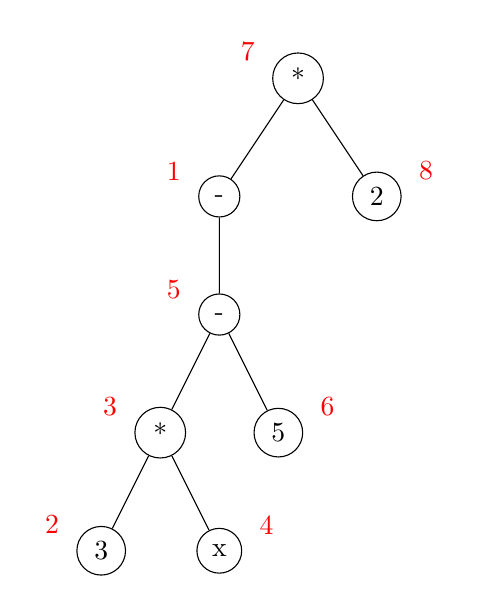
\begin{tikzpicture}[
      level distance=1.5cm,
      level 1/.style={sibling distance=2cm},
      level 2/.style={sibling distance=2cm},
      level 3/.style={sibling distance=1.5cm},
      every node/.style={draw, circle, align=center},
    ]
      \node[label={[label distance=0.1cm, text=red]165:7}] {*}
        child {
          node[label={[label distance=0.1cm, text=red]165:1}] {-}
          child {
            node[label={[label distance=0.1cm, text=red]165:5}] {-}
            child {
              node[label={[label distance=0.1cm, text=red]165:3}] {*}
              child {
                node[label={[label distance=0.1cm, text=red]165:2}] {3}
              }
              child {
                node[label={[label distance=0.1cm, text=red]15:4}] {x}
              }
            }
            child {
              node[label={[label distance=0.1cm, text=red]15:6}] {5}
            }
          }
        }
        child {
          node[label={[label distance=0.1cm, text=red]15:8}] {2}
        };
    \end{tikzpicture}
    \caption{\\Modificeret Inorder Travesal}
  \end{subfigure}
  \hfill
  \begin{subfigure}{0.3\textwidth}
    \centering
    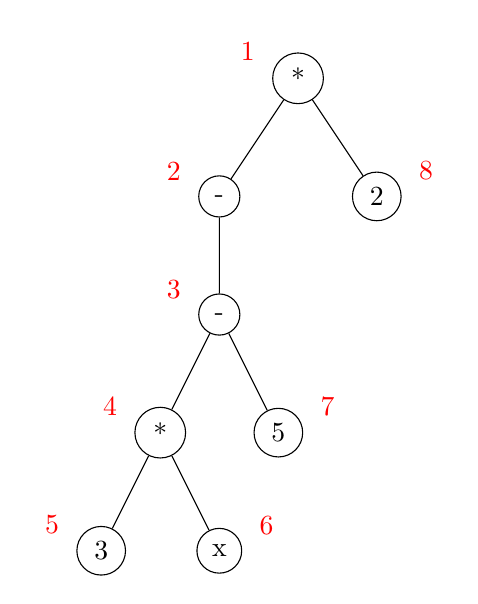
\begin{tikzpicture}[
      level distance=1.5cm,
      level 1/.style={sibling distance=2cm},
      level 2/.style={sibling distance=2cm},
      level 3/.style={sibling distance=1.5cm},
      every node/.style={draw, circle, align=center},
    ]
      \node[label={[label distance=0.1cm, text=red]165:1}] {*}
        child {
          node[label={[label distance=0.1cm, text=red]165:2}] {-}
          child {
            node[label={[label distance=0.1cm, text=red]165:3}] {-}
            child {
              node[label={[label distance=0.1cm, text=red]165:4}] {*}
              child {
                node[label={[label distance=0.1cm, text=red]165:5}] {3}
              }
              child {
                node[label={[label distance=0.1cm, text=red]15:6}] {x}
              }
            }
            child {
              node[label={[label distance=0.1cm, text=red]15:7}] {5}
            }
          }
        }
        child {
          node[label={[label distance=0.1cm, text=red]15:8}] {2}
        };
    \end{tikzpicture}
    \caption{\\Preorder Traversal}
  \end{subfigure}
  \hfill
  \begin{subfigure}{0.3\textwidth}
    \centering
    \begin{tikzpicture}[
      level distance=1.5cm,
      level 1/.style={sibling distance=2cm},
      level 2/.style={sibling distance=2cm},
      level 3/.style={sibling distance=1.5cm},
      every node/.style={draw, circle, align=center},
    ]
      \node[label={[label distance=0.1cm, text=red]165:8}] {*}
        child {
          node[label={[label distance=0.1cm, text=red]165:6}] {-}
          child {
            node[label={[label distance=0.1cm, text=red]165:5}] {-}
            child {
              node[label={[label distance=0.1cm, text=red]165:3}] {*}
              child {
                node[label={[label distance=0.1cm, text=red]165:1}] {3}
              }
              child {
                node[label={[label distance=0.1cm, text=red]15:2}] {x}
              }
            }
            child {
              node[label={[label distance=0.1cm, text=red]15:4}] {5}
            }
          }
        }
        child {
          node[label={[label distance=0.1cm, text=red]15:7}] {2}
        };
    \end{tikzpicture}
    \caption{\\Postorder Traversal}
  \end{subfigure}
  \begin{align*}
      \text{Modificeret Inorder Traversal:} \quad & - (3 \cdot x - 5) \cdot 2 \\
      \text{Preorder Traversal:} \quad &  \cdot - - \cdot 3\, x\, 5\, 2  \\
      \text{Postorder Traversal:} \quad & 3\, x\, \cdot 5\, - -  2\, \cdot
  \end{align*}
  \caption{Træet fra Figur \ref{fig:expression_tree} med forskellige travesal metoder}
  \label{fig:expression_tree_traversal}
\end{figure}


Vi vil i sektion \ref{sec:expression_module} betragte hvordan vi kan implementere et modul, som kan repræsentere udtryk ved brug af prefix notation.
Postorder Traversal bliver blandt andet anvendt til at kunne rekursivt reducere og evaluere udtryk.

Grundet præcedens regler i infix notation, er det nødvendigt at modificere Inorder Traversal, da unære noder altid skal håndteres før dens børn. Desuden vil det også være nødvendigt at implementere regler for at håndtere parenteser, hvis der ønskes et symbolsk udtryk. Den modificerede Inorder Traversal anvendes til at kunne visualisere udtrykket i infix notation.


\subsubsection{Udtryksmodulet}\label{sec:expression_module}
Vi starter med at definere en polymorf type for udtryk, givet i Listing \ref{expr_type}. Denne type omfatter flere konstruktører, hver tilknyttet specifikke matematiske operationer vi ønsker at implementere. Desuden introducerer vi konstruktøren \texttt{N} til at repræsentere numeriske værdier ved at anvende talmængder defineret i Listing \ref{number_type}. Til sidst tilføjer vi konstruktøren \texttt{X} for variable. Således lagres matematiske udtryk som en rekursiv type, der skal repræsentere udtryks træerne i sektion \ref{sec:expression_as_trees}. Dette skyldes at, hver konstruktør for en operation indeholder et eller to underudtryk af samme type.


\begin{lstlisting}[
    language={FSharp}, 
    label={expr_type}, 
    caption={Typen for Expr}
    ]
type Expr<'a> = 
    | X of char
    | N of 'a
    | Neg of Expr<'a>
    | Add of Expr<'a> * Expr<'a>
    | Sub of Expr<'a> * Expr<'a>
    | Mul of Expr<'a> * Expr<'a>
    | Div of Expr<'a> * Expr<'a>
\end{lstlisting}

\texttt{Expr<'a>}  typen er dermed en polymorfisk type, hvor 'a er typen for den talmængde, hvor vi kan lave brugerdefinerede matematiske operationer. Et eksemplar på en \texttt{Expr<Number>}  er givet i Listing \ref{lst:expr_example}. Her ses det, at når udtrykket $-(3 \cdot x - 5) \cdot 2$ visualiseres, er det i prefix notation. 

\begin{lstlisting}[style=output, label={lst:expr_example}, caption={$-(3 \cdot x - 5) \cdot 2$ som et udtryks træ. Funktionen \textcolor{red}{tree} bliver beskrevet i \ref{sec:expression_generation}.}]
> tree "-(3*x-5)*2";;
val it: Expr<Number> = 
  Mul (Neg (Sub (Mul (N (Int 3), X 'x'), N (Int 5))), N (Int 2))
\end{lstlisting}

Signatur filen indeholder overskrivninger på de matematiske operationer, så de kan anvendes på udtryk, samt en funktion \textcolor{red}{eval} til at evaluere et udtryk beskrevet i sektion \ref{sec:eval}. 
\lstinputlisting[
    language=FSharp,
    label={Expression.fsi},
    caption={Signatur filen for Expression modulet}
    ]{../modules/Expression.fsi}



De overskrevne matematiske operatorer i implementeringsfilen for udtryk, laver overfladeevalueringer samt reduceringer på deres respektive argumenter. Overfladeevaluering vil sige, at de individuelle funktioner kun betragter de to øverste niveauer på de udtrykstræer, de tager som argumenter. Implementeringerne af addition og multiplikation er givet i Listing \ref{lst:mul_expr}. Lignende funktioner er implementeret for de andre operationer.

\begin{lstlisting}[
  language={FSharp}, 
  label={lst:mul_expr}, 
  caption={Addition og multiplikation af to udtryk}
  ]
// mul: Expr<Number> -> Expr<Number> -> Expr<Number>
let rec mul e1 e2:Expr<Number> =
  match e1, e2 with
  |N a, N b                       -> N (a * b)
  |N a, b | b, N a when isOne a   -> b
  |N a, _ | _, N a when isZero a  -> N zero
  |Div(a, b), c | c, Div(a, b)    -> Div (mul a c, b)
  |Div (a, b), Div (c, d)         -> Div ((mul a c), (mul b d))
  |Neg a, Neg b                   -> mul a b
  | _, _                          -> Mul(e1, e2)

// add: Expr<Number> -> Expr<Number> -> Expr<Number>
let rec add e1 e2:Expr<Number>  =
  match e1, e2 with
  | N a, N b                            -> N (a + b)
  | N a, b | b, N a when isZero a       -> b
  | a, b when a = b                     -> Mul (N two, b)
  | Neg a, Neg b                        -> neg (add a b) 
  | Neg a, b | b, Neg a                 -> Sub (b, a)
  | Mul(a, X b), Mul(c, X d) 
  | Mul(X b, a), Mul(c, X d)
  | Mul(a, X b), Mul(X d, c) 
  | Mul(X b, a), Mul(X d, c) when b = d -> Mul(add a c, X b)
  | _, _                                -> Add(e1, e2)

\end{lstlisting}

\subsection{Evaluering af udtryk}\label{sec:eval}
Vi begynder med at definere et miljø, som værende en samling af variable og deres tilhørende værdier. 
Vi vil nu betragte, hvordan vi kan evaluere et udtryk, ved hjælp af et miljø. Evalueringen af udtryk skal kunne opfylde følgende homomorfiske egenskaber \ref{prop:eval_homomorphism}. Egenskaben vil blive valideret i sektion \ref{sec:PBT_eval_homomorphism}.
\vspace{0.5cm}
\begin{egenskab}[Homomorfisme af evaluering]\label{prop:eval_homomorphism}
Lad $\oplus \in \{+, -, \times, /\}$ sættet af binære operationer, $e1$ og $e2$ være udtryk, samt "env" være et miljø, som indeholder værdier for de variable, der er indeholdt i $e1$ og $e2$, så gælder følgende:
\begin{align*}
    \text{eval}(e1 \oplus e2, \text{env}) = \text{eval}(e1, \text{env}) \oplus \text{eval}(e2, \text{env})
\end{align*}
Derudover skal det om negation også gælde at:
\begin{align*}
    \text{eval}(-e1, \text{env}) = -\text{eval}(e1, \text{env})
\end{align*}
\end{egenskab}


Funktionen \textcolor{red}{eval} i Listing \ref{lst:eval_expr} tager et udtryk og et miljø som input og evaluerer udtrykket til en numerisk værdi. Funktionen kører en Postorder Traversal på udtrykket og evaluerer dermed udtrykket nedefra og op, ved at foretage matematiske operationer defineret i \texttt{Number} modulet. 

\begin{lstlisting}[
  language={FSharp}, 
  label={lst:eval_expr}, 
  caption={Evaluering af et udtryk}
  ]
// eval: Expr<Number> -> Map<char, Number> -> Number
let rec eval (e:Expr<Number>) (env) =
  match e with
  | X x -> Map.find x env
  | N n -> n
  | Neg a -> - eval a env
  | Add (a, b) -> eval a env + eval b env
  | Sub (a, b) -> eval a env - eval b env
  | Mul (a, b) -> eval a env * eval b env
  | Div (a, b) -> eval a env / eval b env
\end{lstlisting}

\subsection{Konventering mellem udtryksformer}\label{sec:expression_generation}
Det ønskes at kunne konvertere udtryk frem og tilbage mellem prefix notation, repræsenteret af Expression-typen, og standard infix notation. Dette ønske skyldes, at infix notation er lettere for os at læse og skrive. Derfor er det essentielt, at de to konverteringsfunktioner fungerer som hinandens inverse. Dette krav er yderligere uddybet i egenskab \ref{egenskab:infix_prefix}. Egenskaben bliver valideret i sektion \ref{sec:PBT_infix_prefix}.

\vspace{0.5cm}
\begin{egenskab}[Invers morphism\footcitetitle{Inverse_function} mellem infix og prefix]\label{egenskab:infix_prefix}
    Lad $Q^n$ være mængden af rationelle infix udtryk med gyldig matematisk notation, som kun indeholder operationer indeholdt i $\{+, -, \times, /\}$, med $n$ variable, så defineres følgende:
    \begin{align*}
      \text{tree}&: Q^n \to \text{Expr} \\
      \text{tree}^{-1}&: \text{Expr} \to  Q^n  
    \end{align*}
    Dermed gælder følgende egenskaber
    \begin{align*}
      \text{tree}^{-1} \circ \text{tree} &= id_{Q^n} \\
      \text{tree} \circ \text{tree}^{-1} &= id_{\text{Expr}}
    \end{align*}
    Hvor $id_{x}$ er identitetsfunktionen på mængden $x$.
\end{egenskab}

Vi begynder med at betragte den inverse funktion, som konverterer et udtryk til infix notation. Funktionen \textcolor{red}{etf} i Listing \ref{lst:expression_to_infix} fortager denne konvertering ved at lave den modificerede Inorder Traversal på udtrykket, som blev beskrevet i sektion \ref{sec:expression_as_trees}. Den modificerede del er at håndtere parenteser samt negation. Dette gøres ved at betragte negation som en node i træet, hvor det venstre barn er et tomt udtryk.

\begin{lstlisting}[
  language={FSharp}, 
  label={lst:expression_to_infix}, 
  caption={konventering fra expression til infix notation}
  ]
// parenthesis: bool -> string -> string
let parenthesis b f = if b then "(" + f + ")" else f

// etf: Expr<Number> -> bool -> string
let rec etf e p =
    match e with
    | N a when not <| isInt a -> toString a |> parenthesis p
    | N a -> toString a
    | X a -> string a
    | Neg a ->  "-" + etf a (not p) |> parenthesis p
    | Add(a, b) -> etf a false + "+" + etf b false |> parenthesis p
    | Sub(a, b) -> etf a false + "-" + etf b true |> parenthesis p
    | Mul(a, b) -> etf a true  + "*" + etf b true |> parenthesis p
    | Div(a, b) -> etf a true  + "/" + etf b true |> parenthesis p

// infixExpression: Expr<Number> -> string
let infixExpression e = etf e false
\end{lstlisting}

Funktionen \textcolor{red}{\texttt{tree}}, som foretager konverteringen fra infix notation til et udtrykstræ, er baseret på algoritmen beskrevet i \cite{convert_expression}\footcitetitle{convert_expression}. Først konverteres en udtryksstreng til en liste af tokens. Disse tokens beskriver, om en karakter i udtrykket er en operand, en operator, eller en konstant, hvor en operator også indeholder information om præcedens og associativitet\footcitetitle{precedens_associativity}. Typen for disse tokens kan ses i Listing \ref{lst:infix_to_expression_types}. Herefter anvendes to stacks: en for operatorer og en for udtryk. Der anvendes en række regler, som beskrevet i \cite{convert_expression}, for hvornår der skal udføres pop og push på disse to stacks. Det skal bemærkes, at når en operator pushes til udtryksstacken, da navnet på operatorkonstruktøren på udtrykket står skrevet fra venstre mod højre, vil udtryksstacken være i prefix notation og ikke postfix notation som beskrevet i kilden. Funktionen \textcolor{red}{\texttt{tree}} er at finde i Appendiks \ref{sec:treeGenerator.fs}.

\begin{lstlisting}[
  language={FSharp}, 
  label={lst:infix_to_expression_types}, 
  caption={Konvertering fra infix til udtrykstræ}
]
type Associative = | Left | Right
type Precedence = int
type Operator = char * Precedence * Associative
type Token =
    | Operand of char
    | Operator of Operator
    | Constant of int
type OperatorList = Operator list
\end{lstlisting}




\subsection{Reducering af udtryk} \label{sec:simplification_expression}
Vi skal nu betragte en systematisk metode til at kunne reducere matematiske udtryk, ved hjælp af simple algebraiske regler. Dette er en nødvendighed at kunne, for at bruge udtrykkene i en matematisk sammenhæng, da det vil kunne medføre både en reduktion i kompleksitet og en forbedring i læsbarhed når udtrykkene visualiseres. Før vi betragter metoden, kan vi opskrive en egenskab som reduceringen skal overholde. Egenskaben \ref{egenskab:simplification} vil blive valideret i sektion \ref{sec:PBT_simplification}, det er en nødvendighed at evaluere udtrykket før og efter reduktion, da det er en kompleks opgave at skulle sammenligne om to udtryk er ækvivalente.
\vspace{0.5cm}
\begin{egenskab}[Reducering af udtryk]\label{egenskab:simplification}
Lad $e$ være et udtryk samt "env" være det miljø som indeholder værdier for variable i $e$, så gælder følgende:
\begin{align*}
  \text{eval}(e, \text{env}) = \text{eval}(\text{simplifyExpr}(e), \text{env})
\end{align*}
\end{egenskab}  

Vi begynder med at betragte funktionen \textcolor{red}{\texttt{simplifyExpr}} i Listing \ref{lst:simplify_expr}, som reducerer et udtryk ved at foretage en Postorder Traversal på udtrykket. Hvilket betyder, at når en node i udtrykstræet skal reduceres, vil dens børn allerede være reduceret. 

\begin{lstlisting}[
  language={FSharp}, 
  label={lst:simplify_expr}, 
  caption={Reducering af et udtryk}
  ]
//simplifyOperation: Expr<Number> -> Expr<Number> -> (Expr<Number> -> Expr<Number> -> Expr<Number>) -> Expr<Number>
let rec simplifyOperation e1 e2 f = 
  match f e1 e2 with
  | Neg a -> 
    commutativeMulDiv.applyCommutative (Neg a) |> commutativeAddSub.applyCommutative
  | Add(a, b) when isAdd f -> commutativeAddSub.applyCommutative (Add(a, b))
  | Sub(a, b) when isSub f -> commutativeAddSub.applyCommutative (Sub(a, b))
  | Mul(a, b) when isMul f -> commutativeMulDiv.applyCommutative (Mul(a, b))
  | Div(a, b) when isDiv f -> commutativeMulDiv.applyCommutative (Div(a, b))
  | Add(a, b) -> simplifyOperation a b (+)
  | Sub(a, b) -> simplifyOperation a b (-)
  | Mul(a, b) -> simplifyOperation a b (*)
  | Div(a, b) -> simplifyOperation a b (/)
  | a -> a

//simplifyExpr: Expr<Number> -> Expr<Number>
let rec simplifyExpr e =
  match e with
  | N a when Number.isNegative a -> Neg (N (Number.absNumber a))
  | N (Rational(R(a, b))) -> 
    simplifyOperation (simplifyExpr (N (Int a))) (simplifyExpr (N (Int b))) (/)
  | Neg a     -> - (simplifyExpr a)
  | Add(a, b) -> simplifyOperation (simplifyExpr a) (simplifyExpr b) (+)
  | Sub(a, b) -> simplifyOperation (simplifyExpr a) (simplifyExpr b) (-)
  | Mul(a, b) -> simplifyOperation (simplifyExpr a) (simplifyExpr b) (*)
  | Div(a, b) -> simplifyOperation (simplifyExpr a) (simplifyExpr b) (/)
  | _ -> e 
\end{lstlisting}

Det er \textcolor{red}{simplifyOperation}, som foretager selve reduceringen af et givet udtryk. Funktionen tager som argumenter to udtryk, samt den binære operation, der skal anvendes på disse. Funktionen anvendes på udtrykkene, hvorefter overfladisk reducering, som blev beskrevet i sektion \ref{sec:expression_module}, udføres. Hvis overfladisk reducering resulterer i en ændring af den anvendte operation, kalder funktionen sig selv rekursivt med de to udtryk og den nye operation. Hvis overfladisk reducering ikke resulterer i ændringer i operationen, vil funktionen foretage en dybere reducering af de to udtryk. Denne dybere reducering udføres af funktionerne \textcolor{red}{applyCommutative} fra filerne \textit{CommutativeAddSub.fs} og \textit{CommutativeMulDiv.fs}, som findes i Appendiks \ref{sec:commutativeAddSub.fs} og \ref{sec:commutativeMulDiv.fs}. Disse funktioner arbejder efter samme princip, hvor de starter med at flade udtrykstræerne ud ifølge de kommutative regler for henholdsvis addition og multiplikation. Derefter sorterer de udtrykstræet, hvilket muliggør at foretage overfladisk simplifikation når træet gendannes. For multiplikation anvendes samme metode i nævneren for division, og der undersøges, om der er fælles udtryk i det udfladede træ, som fremtræder i nævneren af en division og i det udfladede træ, der indeholder divisionen. Et eksempel på anvendelse af den kommutative multiplikationsreducering på et udtryk er givet i Figur \ref{fig:expression-trees}, som viser det visuelle input og det resulterende svar fra funktionen, samt Figur \ref{fig:trees}, der viser det udfladede træ og sorteringen af det fladede træ.


\begin{figure}[H]
  \centering
  \begin{subfigure}[b]{0.5\textwidth}
    \centering
    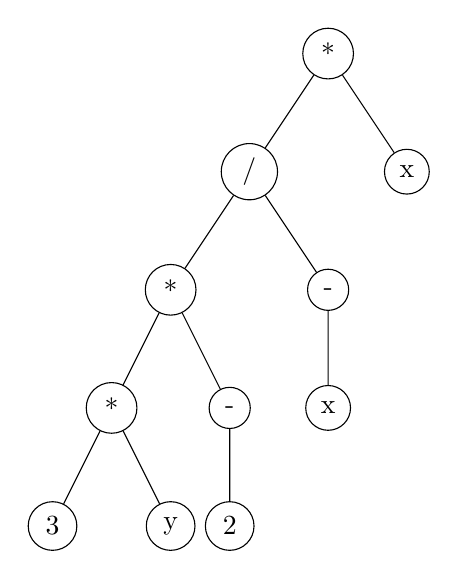
\begin{tikzpicture}[
      level distance=1.5cm,
      level 1/.style={sibling distance=2cm},
      level 2/.style={sibling distance=2cm},
      level 3/.style={sibling distance=1.5cm},
      every node/.style={draw, circle, align=center},]
      \node {*}
        child { node {/}
          child { node {*}
            child { node {*}
              child { node {3}
              }
              child { node {y}
              }
            }
            child { node {-}
              child { node {2}
              }
            }
          }
          child { node {-}
            child { node {x}
            }
          }
        }
        child { node {x}
        };
    \end{tikzpicture}
    \caption{Udtrykket $(3 \cdot y \cdot (-2)/-x) \cdot x$ som et træ}
    \label{fig:original-tree}
  \end{subfigure}
  \hfill
  \begin{subfigure}[b]{0.4\textwidth}
    \centering
    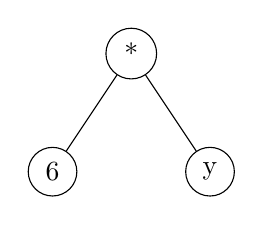
\begin{tikzpicture}[
      level distance=1.5cm,
      level 1/.style={sibling distance=2cm},
      every node/.style={draw, circle, align=center},]
      \node {*}
        child { node {6} }
        child { node {y} };
    \end{tikzpicture}
    \caption{Det resuterende reduceret udtryk, efter at have anvendt CommutativeMulDiv.\textcolor{red}{applyCommutative} på udtrykket i Figur \ref{fig:original-tree}}
    \label{fig:simplified-tree}
  \end{subfigure}
  \caption{Før og efter reducering af et udtryk ved brug af CommutativeMulDiv.\textcolor{red}{applyCommutative}}
  \label{fig:expression-trees}
\end{figure}


% Flattened Tree
\begin{figure}[H]
  \centering
  \begin{subfigure}[b]{0.45\textwidth}
    \centering
    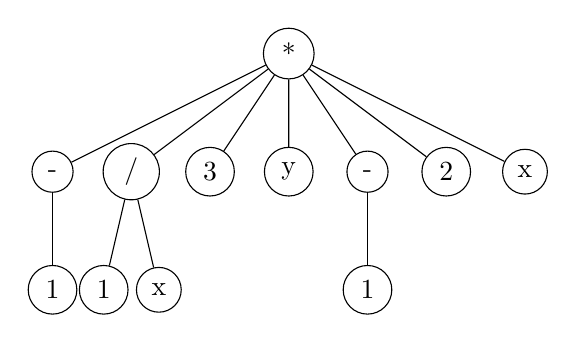
\begin{tikzpicture}[level distance=1.5cm,
      level 1/.style={sibling distance=1cm},
      level 2/.style={sibling distance=0.7cm},
      level 3/.style={sibling distance=1.5cm},
      every node/.style={draw, circle, align=center},]89
      \node {*}
        child{ node {-} 
          child { node {1}}}
        child { node {/}
          child { node {1}
          }
          child { node {x}}
        }
        child { node {3}
        }
        child { node {y}
        }
        child { node {-}
          child { node {1}
          }
        }
        child { node {2}
        }
        child { node {x}
        };
    \end{tikzpicture}
    \caption{Det udfladede træ}
    \label{fig:sub1}
  \end{subfigure}
  \hfill
  \begin{subfigure}[b]{0.45\textwidth}
    \centering
    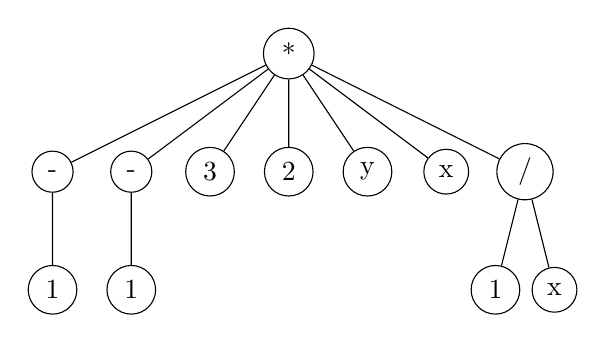
\begin{tikzpicture}[level distance=1.5cm,
      level 1/.style={sibling distance=1cm},
      level 2/.style={sibling distance=0.75cm},
      level 3/.style={sibling distance=1cm},
      every node/.style={draw, circle, align=center},]
      \node {*}
        child { node {-}
          child { node {1} }
        }
        child { node {-}
          child { node {1} }
        }
        child { node {3} }
        child { node {2} }
        child { node {y} }
        child { node {x} }
        child { node {/}
          child { node {1} }
          child { node {x} }
        };
    \end{tikzpicture}
    \caption{Det sorterede træ fra venstre mod højre}
    \label{fig:sub2}
  \end{subfigure}
  \caption{Det udfladede og sorterede af udtrykket $(3 \cdot y \cdot (-2)/-x) \cdot x$ i processen af kommutativ reducering}
  \label{fig:trees}
\end{figure}

Generelt, når det gælder reducering af udtryk, skal man være opmærksom på ikke at ende i et uendeligt loop. Derfor er det vigtigt ikke at definere nogle overfladiske reduceringer, som er hinandens inverse funktioner. Desuden forsøger funktionerne i dette program altid at skubbe negation af udtryk så langt ud som muligt i håb om, at de kan ophæve hinanden. Dette illustreres blandt andet i figur \ref{fig:trees}, hvor ved udfladning af træet, hvis et af de kommutative udtryk for multiplikation er negativt, fjernes negationen, og der tilføjes i stedet en negation af tallet 1, som ved sortering skubbes til venstre.


\subsection{Differentiation af udtryk}
Vi kan nu betragte den første implementering, der benytter vores udtryksmodul, som samtidig vil understrege vigtigheden af at kunne reducere udtryk. Vi begynder igen med at opskrive nogle algebraiske linearitetsegenskaber, som differentieringen skal overholde. Disse egenskaber vil blive testet i sektion \ref{sec:PBT_differentiation}.
\vspace{0.5cm}
\begin{egenskab}[Linearitetsbetingelserne\footcitetitle{diff}]\label{egenskab:differentiation}
  Lad $f$ og $g$ være udtryk, og $a$ være tal fra talmodulet, så gælder følgende:
  \begin{enumerate}
    \item \textbf{Skaleringsreglen} \\
    \(\frac{d}{dx}(af) = a\frac{df}{dx}\)
    \item \textbf{Sumreglen} \\
    \(\frac{d}{dx}(f+g) = \frac{df}{dx} + \frac{dg}{dx}\)
    \item \textbf{Subtraktionsreglen} \\
    \(\frac{d}{dx}(f-g) = \frac{df}{dx} - \frac{dg}{dx}\)
    \item \textbf{Produktreglen} \\
    \(\frac{d}{dx}(fg) = \frac{df}{dx}g + f\frac{dg}{dx}\)
    \item \textbf{Kvotientreglen} \\
    \(\frac{d}{dx}\left(\frac{f}{g}\right) = \frac{\frac{df}{dx}g - f\frac{dg}{dx}}{g^2}\)
  \end{enumerate}
\end{egenskab}

Funktionen for differentiering \textcolor{red}{diff} i Listing \ref{lst:diff_expr}, tager et udtryk og en variabel som input og differentierer udtrykket med hensyn til variablen. Dette er en af de store fordele ved at anvende et funktionelt programmeringssprog, da det ses hvordan reglerne fra egenskab \ref{egenskab:differentiation} er implementeret direkte, som de er beskrevet.

\begin{lstlisting}[
  language={FSharp}, 
  label={lst:diff_expr}, 
  caption={Differentiering af et udtryk}
  ]
// diff: Expr<Number> -> char -> Expr<Number>
let rec diff e dx = 
    match e with
    | X f when f = dx -> N (Int 1)
    | X _ -> N (Int 0)
    | N _ -> N (Int 0)
    | Neg f -> Neg (diff f dx)
    | Add(f, g) -> Add(diff f dx, diff g dx)
    | Sub(f, g) -> Sub(diff f dx, diff g dx)
    | Mul(f, g) -> Add(Mul(diff f dx, g), Mul(f, diff g dx))
    | Div(f, g) -> Div(Sub(Mul(diff f dx, g), Mul(f, diff g dx)), Mul(g, g))
\end{lstlisting}

At differentiere et udtryk vil blandt andet resultere i mange nul værdier i det resulterende udtryk, hvortil simplifikation efter differentiering vil være en fordel.


\subsection{Multivariable polynomier af første grad}
Da vi senere i projektet skal betragte matricer, vil vi i den forbindelse også lave en løsning af lineære ligningssystemer i sektion \ref{sec:lin_eq}. Det kræver derfor, at vi kan isolere variable i et multivariabelt polynomium af første grad. Vi betragter derfor nu to simple funktioner til at udføre denne isolation, se Listing \ref{lst:isolate}. Funktionen \textcolor{red}{isolateX} undersøger først, om den variabel, som skal isoleres, befinder sig på højre eller venstre side. Derefter kaldes funktionen \textcolor{red}{expressionOnX}, som fungerer ved at evaluere til en funktion, der giver den omvendte operation af den operation, som variablen er involveret i. Dertil anvendes den omvendte funktion på begge sider af ligningen, hvor hvis variablen er isoleret, gives et udtrykspar, hvor det første udtryk er den isolerede variabel. Hvis variablen ikke er isoleret, kaldes funktionen rekursivt med de nye højre og venstre sider.

\begin{lstlisting}[
  language={FSharp}, 
  label={lst:isolate}, 
  caption={Isolering af variable i et udtryk}
  ]
// expressionOnX: Expr<'a> -> Expr<'a> -> (Expr<'a> -> Expr<'a>)
let rec expressionOnX hs x =
  match hs with
  | N _ | X _ -> fun e -> e
  | Neg(a) when a = x -> fun e -> Neg e
  | Sub(a, b) when a = x -> fun e -> Add(e, b)
  | Div(a, b) when a = x -> fun e -> Mul(e, b)
  | Div(_, a) when a = x -> fun e -> Mul(e, a)
  | Mul(a, b) | Mul(b, a) when a = x -> fun e -> Div(e, b)
  | Add(a, b) | Add(b, a) | Sub(b, a) when a = x -> fun e -> Sub(e, b)
  | Add(a, b) | Sub(a, b) | Mul(a, b) | Div(a, b) -> fun e -> expressionOnX a x e |> expressionOnX b x 
  | Neg(a) -> fun e -> expressionOnX a x e

// isolateX: Expr<Number> -> Expr<Number> -> Expr<Number> -> Expr<Number> * Expr<Number> 
let rec isolateX lhs rhs x =
  let operation = 
      if containsX lhs x 
          then expressionOnX lhs x
      elif containsX rhs x 
          then expressionOnX rhs x
      else 
          failwith "Variable not found in either side of the equation"
  match operation lhs |> simplifyExpr, operation rhs |> simplifyExpr with
  | a, b | b, a when a = x -> (a, b)
  | a, b -> isolateX a b x
\end{lstlisting}

Da funktionen kun betragter operationen på den variable, der ønskes isoleret, eksisterer der mange tilfælde, hvor funktionen ikke vil kunne isolere variablen. Men den fungerer til at løse ligninger af formen \(a_1x_1 + a_2x_2 + \ldots + a_nx_n = b\), hvilket er tilstrækkeligt for vores formål.
